\section{Discussion}

The promise of 3D printing is that it allows for the manufacture of geometries that are impossible to create using traditional techniques like injection molding.  Pipes leverage that promise: designing the internal structure of an object was not previously feasible. \bjoern{overly broad claim. companies are designing the "interior " when they make complex shelled parts using injection molding. But that process has lots of limitations as to the geometries that are possible --- there's a whole industry of specialists concerned with ``design for manufacturability'' (DFM).} As printers at the hobbyist and corporate levels become more sophisticated and able to fabricate intricate geometries of ever more materials, we believe that our tool will still assist in design tasks. \bjoern{oblique, and could be phrased more positively.} Even if printers are capable of laying down conductive, optically transparent, or luminescent materials in-place, the process of designing their paths is still crucial.

By crossing pipe types, topologies, and inserted media, we create a space of possible inputs and outputs that can be pipe-mediated.  We arrange our I/O discussion  around the modes of input or output (the five senses, touch/tapping/pressure/etc.).  We also suggest new points in the design space of pipe-mediated interaction that remain unexplored. \bjoern{need to motivate first why the discussion is going to focus on inputs and outputs - why is this the logical topic to return to? Maybe something like this: ``By crossing pipe types, topologies, and inserted media, many pipe-mediated interactions emerge. We demonstrated a few such possibilities by designing and fabricating example objects with the help of our pipe routing design tool. However, there are many additional possibilities for leveraging sensing and actuation techniques from the HCI literature and extending their use in 3D-printed objects. We briefly survey such possibilities for output and input.''}

\subsection{Outputs}

Pipe-based outputs can address the five senses: visual, aural, haptic, and olfactory/gustatory.  In addition to outputs we mention explicitly, any outputs possible using traditional electronic components are possible using conductive material in pipes.

\begin{figure}[h]
\centering
    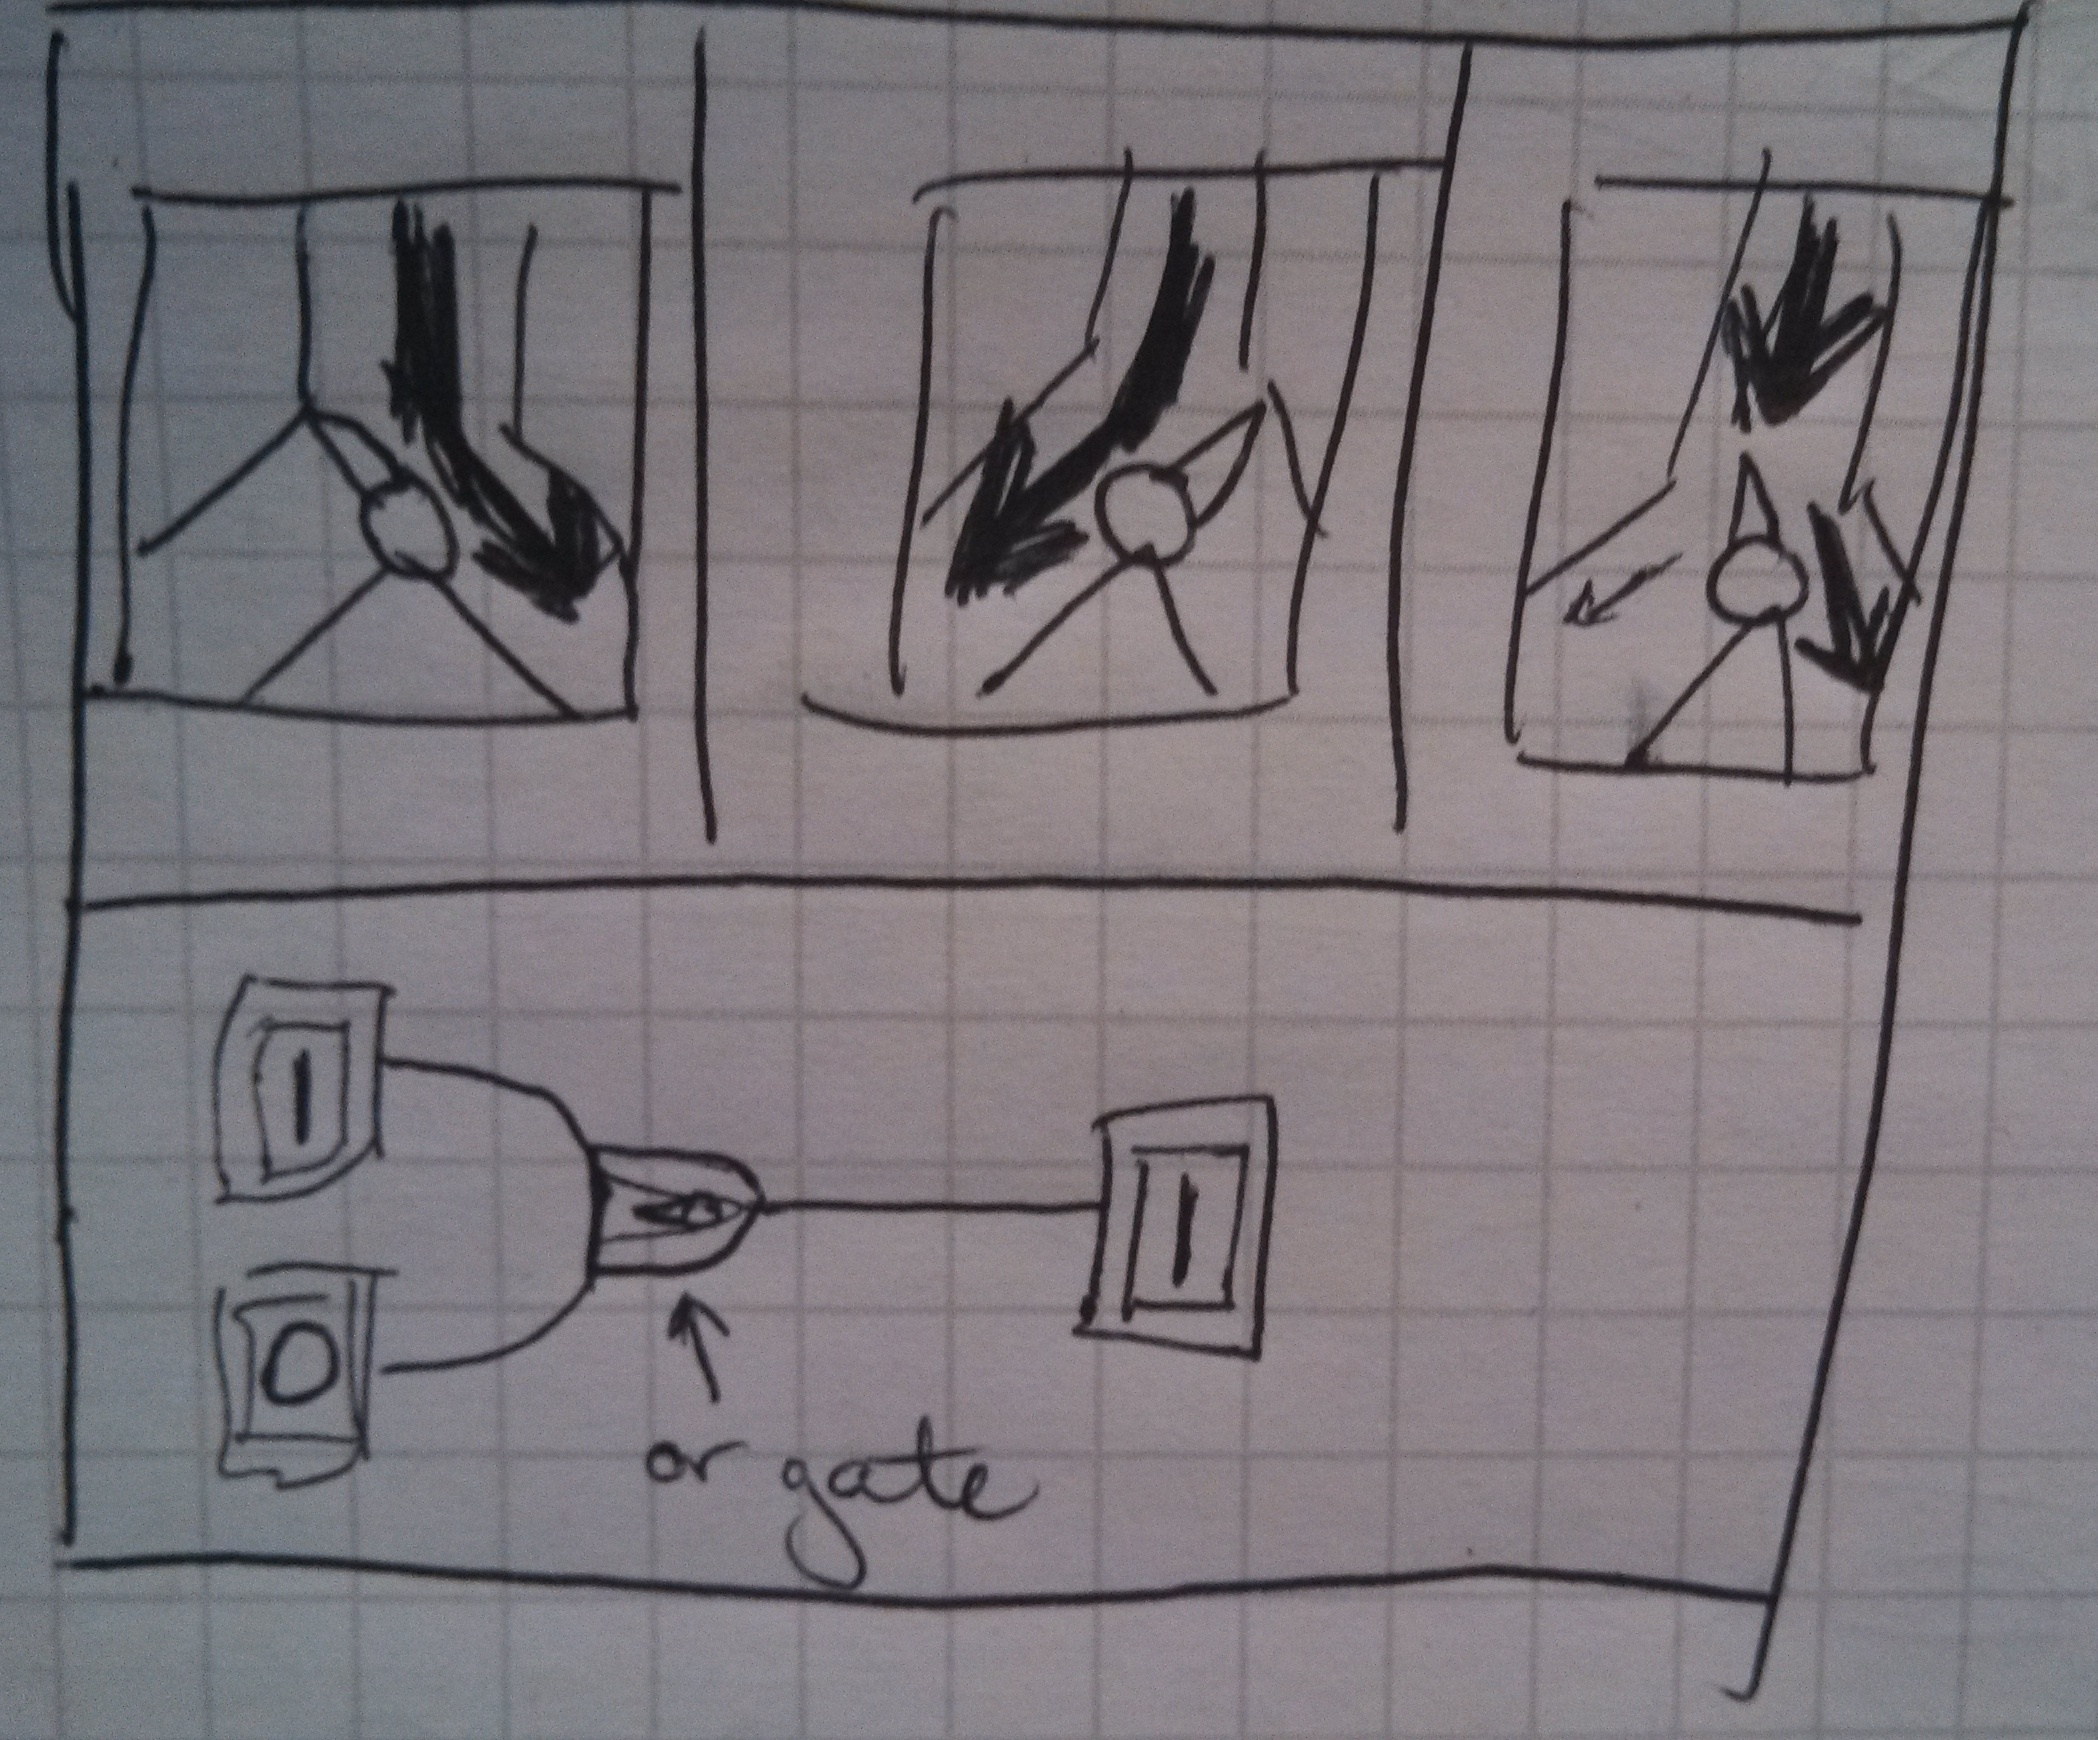
\includegraphics[width=3.4in]{figures/placeholder/direct.jpg}
\caption{By attaching a servo to a gate structure, it is possible to direct fluid through that pipe.  The gate not only has binary positions (a) and (b), but can direct fractional flow, as well (c).  This could be used to create logic gates, as in (d).  These could be used, for example, in science exhibits.}
\label{fig:direct}
\end{figure}

\emph{Visual} outputs can be mediated by gases, liquids, solid, particulates, or threadables.  Pneumatic actuation (as in PneUIs \cite{Yao-pneui} or Harrison's latex buttons \cite{Harrison-buttons}) provides output, but gases carrying smoke (as in the Aireal \cite{Sodhi-aireal} demo) also offers visual feedback \bjoern{mischaracterization of aireal - they only added smoke to show what a vortex looks like; the technique is all about invisible, haptic sensation}.  Splitting and mixing of colored liquids can be used as a display tactic; additionally mechanical motion can be fluid-mediated.  Liquids can also be mixed in specific concentrations by servo-controlled gate structures as in Figure \ref{fig:direct}.  Printed optics \cite{Willis-printedoptics} explored visual output at the ends of pipes, and  EL wire can be threaded through custom paths to create neon signs, as in our neon robot (Figure \ref{fig:neon}) \bjoern{are we going to repeat things here we already talked about? Maybe we should just focus on ideas one could build that we haven't built yet}.

\emph{Aural} outputs can be created with gases.  Helmholz resonance can be leveraged to create computer-controllable sound chambers, as in Zoran's flute \cite{Zoran-flute}.  All that is necessary for this is an enclosed chamber with a pipe connected to it via a narrow neck-point (see Figure \ref{fig:ocarina}).  Passive sound amplification and sound redirection are also possible using pipes.

\begin{figure}[h]
\centering
    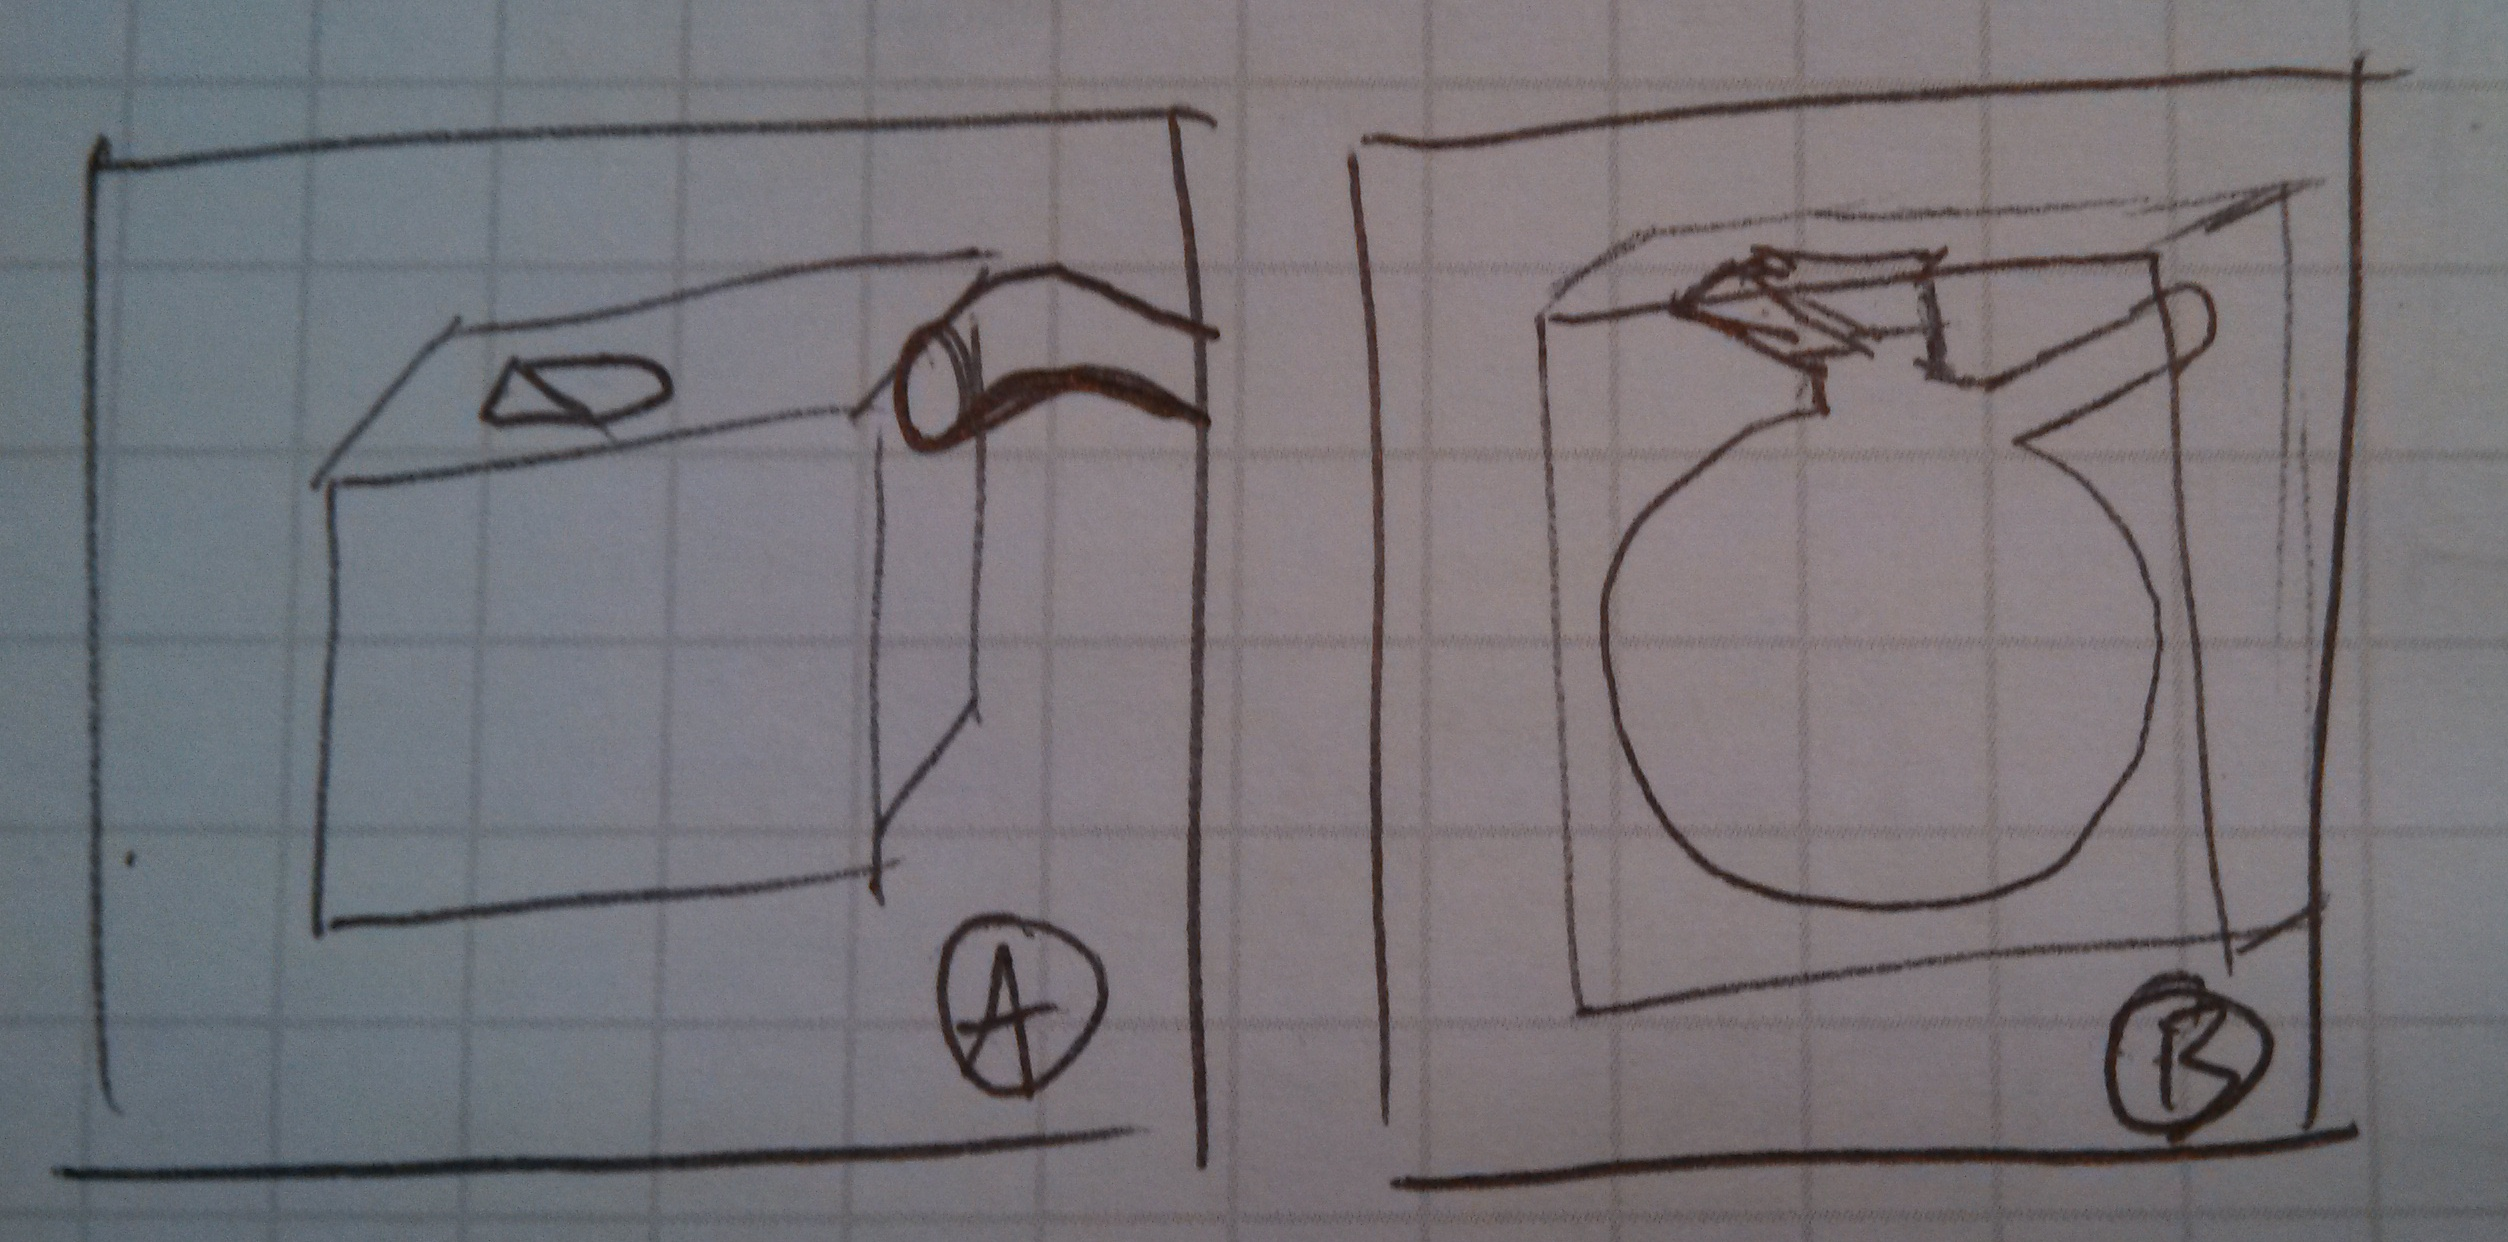
\includegraphics[width=3.4in]{figures/placeholder/helmholz.jpg}
\caption{This box (a) contains an enclosed Helmholz resonator, seen in the cutaway view (b).  This resonator creates a sound when air is blown through the pipe at the top, because air compresses at the small neck joint between the chamber and the pipe.  \valkyrie{need to get a test print of this that actually works}}
\label{fig:ocarina}
\end{figure}

\emph{Haptic} outputs are possible through compressible and incompressible fluids.  Fluids in pipes capped with flexible membranes can actuate particulates and create programmable pliability as in Jamming User Interfaces \cite{Follmer-jamming}.  Additionally, use of semi-closed pipes with rubberlike material as the caps allows for gases to actuate surface features, like the back of our breathing rabbit (see Figure \ref{fig:breathe}).  Free-air haptic feedback as in Aireal \cite{Sodhi-aireal} and volumetric interactions as in Volflex \cite{Iwata-volflex} can also be pipe-mediated.

\emph{Olfactory} and \emph{gustatory} outputs can be created through the mixing and splitting of pipes carrying scented or flavored fluids, respectively.

\subsection{Inputs}

Pipes create opportunities for many types of input sensing across the surface of printed devices.  We describe sensing touch, pressure, grasp, flexing, tapping, and manipulation of traditional electronic components.  There are likely more input sensing techniques, both existing and on the horizon, that are compatible with the use of pipes.

\emph{Touch} sensing can be enabled through pipes filled with conductive media.  Traditional wires (threadable) may be used, but conductive paint (liquid) may be more flexible.  Using conductive paint and Swept Frequency Capacitive Sensing (SFCS \cite{Sato-touche}), an interior star pipe topology can enable single-wire touch- and grasp-sensing at any set of points on a printed object's surface, like our toys (see Figure \cite{fig:toys}).  Simple capacitance measurements are possible using the same media, and custom-designed sensors like those created in Savage, et al.,'s Midas system are also possible \cite{Savage-midas}.  Using a technique like Fiberio \cite{Holz-fiberio}, users could even be identified on touches.

\emph{Pressure} can be sensed in multiple ways.  Slyper, et al.,'s primitives can be attached as the terminus of any semi-closed pipe; the user can manipulate the printed endpoint and the system can sense air pressure changes \cite{Slyper-pressure}.  Pressure can also be sensed via capacitance.

\emph{Grasp} sensing can be enabled using Wimmer's FlyEye techniques \cite{Wimmer-flyeye} or those described in Jamming User Interfaces \cite{Follmer-jamming}.  The optical links necessary for sensing can be created either via clear solid cores as in Printed Optics \cite{Willis-printedoptics} or via fiber optic cables threaded through hollow pipes (see Figure \ref{fig:pens}).

Some 3D printers can fabricate rubber-like materials.  Similar to Slyper, et al., in \cite{Slyper-shape}, we can sense \emph{flexing} and \emph{bending} of prints made on these machines: the ability to 3D print devices to sensing bending and flexing significantly cuts molding and assembly time.

\emph{Tapping} is another input possibility.  Due to differential sound conductivity in different printed materials, pipes of a greater conducting material can be embedded in a model of a lesser conducting material.  A microphone or piezo placed at the system-side of these sound-conducting pipes can determine where the model was tapped and how it was tapped.  Active acoustic sensing as described in Touch \& Activate \cite{Ono-touchandactivate} is also possible; this technique would allow for particular areas of interest (connected to sound-conducting pipes) to be touch sensitive, while other areas (made of non-conducting material) are not sensed.

Sensing via traditional electronic components (e.g., potentiometers, alcohol gas sensors) can be accomplished by conductive inserted media.  Components can be recessed into a print's surface, with their leads implanted into open pipes.  By inserting liquid copper paint instead of threading traditional wires, all components in a model can share a ground line, and the paint's drying process obviates the use of solder or glue to affix the components in place (see Figure \ref{fig:radio}).

\subsubsection{Identification}
In addition to active inputs from users, pipes can be used for passive \emph{identification}.  While the pipes need not be visible (especially in the case of fully-enclosed pipes), their presence, location, network structure, and length change the physical properties of a printed object.  This includes weight, acoustic resonance, and (if conductive material is present) capacitive signature.

Both identification by recall and intentional encoding are possible.  As seen in \cite{Ono-touchandactivate}, different objects have different acoustic signatures.  Additionally, two objects that are visually identical but which have fully enclosed (or other types) of pipes on their interior can be distinguished acoustically.  Thus we can recall an object's identity once its acoustic signature has been recorded.  Similarly, the Touch\'{e} system in \cite{Sato-touche} relies on distinguishing capacitive signatures of objects, both in static states and as their boundary conditions are changed by human interaction.  Weight is a simple metric of object identity, but weights are less distinctive than acoustic or capacitive signatures, as they are represented by a single number.

We have also experimented with intentional encoding.  Semi-closed pipes can function as resonance chambers.  An object's resonant frequency can be measured by attaching a speaker and microphone to it, sweeping frequencies with the speaker, and performing a Fourier transform on the resultant signal from the microphone.  Peaks in the transformed data correspond to stronger returned impulses: the resonant frequencies of the object.  Intentional encoding in the case of capacitance is significantly more difficult, and we leave it to future work.  Encoding of weight is trivial by creating fully-enclosed chambers inside an object.

This is similar to work done by Willis, et al., in \cite{Willis-infrastructs}.  While their technique requires access a terahertz imaging tool, audio resonance identity encoding requires only a microphone and a speaker.

\bjoern{We might pull back on the scope of this section a bit and think about which directions here are most closely related to pipes and most likely successful;  and which are more tangential or speculative - for example, Aireal is about feedback in free space and we are all about designing tangible objects; so maybe that's a candidate for cutting.}